\nsection{Dynamic programming}

\subsection{All submasks of a mask }
\begin{code}
  for (int B = A; B > 0; B = (B - 1) & A)
\end{code}

\subsection{Broken profile \complexity{n \cdot m \cdot 2^n} with $n \leq m$}

Cuenta todas las maneras en las que puedes acomodar fichas de 1x2 y 2x1 en un tablero $n \cdot m$ \\
\addcode{../Codes/Dynamic programming/Broken profile.cpp}

\subsection{Convex hull trick \complexity{n^2} $\Rightarrow$ \complexity{n}}

$ dp[i] = \min_{j < i}(dp[j] + b[j] * a[i]) $ \\
$ dp[i][j] = \min_{k < j}(dp[i - 1][k] + b[k] * a[j]) $ \\
$ b[j] \geq b[j + 1] \text{ optionally } a[i] \leq a[i + 1] $ \\ 
\addcode{../Codes/Dynamic programming/Convex hull trick.cpp}

\subsection{Digit dp }
Counts the amount of numbers in $[l, r]$ such are divisible by $k$. (flag $nonzero$ is for different lengths)  \\
It can be reduced to $dp(i, x, small)$, and has to be solved like $f(r) - f(l - 1)$ \\
\addcode{../Codes/Dynamic programming/Digit dp.cpp}

\subsection{Divide and conquer \complexity{k \cdot n^2} $\Rightarrow$ \complexity{k \cdot nlogn}}

Split the array of size $n$ into $k$ continuous groups. $k \leq n$ \\
$ cost(a, c) + cost(b, d) \leq cost(a, d) + cost(b, c)$ with $a \leq b \leq c \leq d$ \\
\addcode{../Codes/Dynamic programming/Divide and conquer.cpp}

\subsection{Knapsack 01 \complexity{n \cdot MaxW}}

\addcode{../Codes/Dynamic programming/Knapsack 01.cpp}

\subsection{Knuth \complexity{n^3} $\Rightarrow$ \complexity{n^2}}

$ dp[l][r] = \min_{l \leq k \leq r}\{dp[l][k] + dp[k][r]\} + cost(l, r)$ \\
\addcode{../Codes/Dynamic programming/Knuth.cpp}

\subsection{Matrix exponentiation \complexity{n^3 \cdot logn}}

If TLE change \lstinline{Mat} to \lstinline{array<array<T, N>, N>} \\
\addcode{../Codes/Dynamic programming/Matrix exponentiation.cpp}

\subsection{SOS dp }
\addcode{../Codes/Dynamic programming/SOS dp.cpp}

\subsection{Inverse SOS dp }
\addcode{../Codes/Dynamic programming/Inverse SOS dp.cpp}

\subsection{Steiner }
\addcode{../Codes/Dynamic programming/Steiner.cpp}
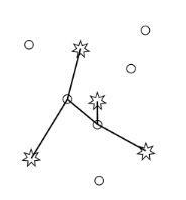
\includegraphics[width=4.5cm]{../Codes/Dynamic programming/SteinerTree.png}
